\documentclass[a4paper]{article}
\usepackage[utf8]{inputenc}
\usepackage[english]{babel}
\usepackage{graphicx}
\usepackage[margin=1.2in]{geometry}
\usepackage{url}

\begin{document}
\baselineskip 13pt

\begin{center}
\section*{\\Internet of Things project\\}
\section*{\\Marco Parola\\}
\end{center}

\clearpage

% ---------- INTRODUCTION -------
\section{Introduction}
This Internet of Things application is developed in order to help parents to monitor their baby's room, integrating a sensor network and a cloud application; all these actions can be performed remotely using the client java application.\\
Using this application the parents can observe their child through a camera installed above the baby cot, moreover they can regulate the light intensity and switch on/off the music.\\


% ---------- ARCHITECTURE -------
\section{Architecture}
The following image shows the architecture of the application:
\begin{center}
\vspace{5mm}
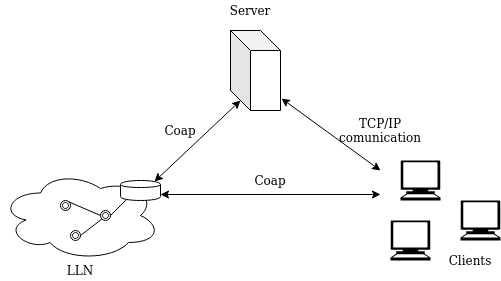
\includegraphics[width=75mm]{architecture.png}
\vspace{5mm}
\end{center}

\subsection{Server}
The server was developed in java. Its main function are:
\begin{itemize}
\item To receive registration request from nodes and keeping track of them.
\item To receive connection request from the clients and handle multithread comunications.
\end{itemize}



\subsection{Client}
This module is developed in java and provide users a command line interface, thanks to which they can interact with other modules (more clients can interact at the same time with the Iot app). In a real scenario this part of the architecture should be a mobile application, which is developed to run on Android and IOs devices (both smartphone and tablet).\\
The following operations can be executed from the users:
\begin{itemize}
\item Swith on/off the camera
\item Read light sensor
\item Switch off/low/medium/high the bulb
\item Read the status of music (on/off)
\item Swith on/off the music
\item Regulate volume of the music
\end{itemize}

\subsection{Nodes}
This module is related to the low power and lossy network. They are written in C programming language and they emulated in cooja simulator. \\
There are 4 types of nodes:
\begin{itemize}
\item rpl border router
\item light node
\item music node
\item camera node
\end{itemize}
A node starts to send a registration request to the server and then it waits for the requests from the clients, providing some methods by which the client can interact with the resources present on the nodes.



\end{document}
